\documentclass{beamer}

\usepackage{cmap}
\usepackage[english,russian]{babel} % add eng,rus(base) package
\usepackage[T1,T2A]{fontenc}        % add eng,rus encoding support
\usepackage[utf8]{inputenc}         % add UTF8 support

% Use it for English document
%\usepackage[utf8]{inputenc} % add UTF8 support
%\usepackage{fontspec}       % to use any font known to the operating system
%\setmainfont{PT Serif}      % set defolt font

\usepackage{amsmath, amsfonts, amssymb, amsthm, mathtools} % add math support

\linespread{1}               % length between str
\setlength{\parindent}{16pt} % red str
\setlength{\parskip}{6pt}   % length between paragraphs

\usepackage[backend=biber, style=authoryear-icomp]{biblatex}
\addbibresource{$HOME/latex-templates/biblio.bib}            % path to bibliography base

\usetheme{Madrid}
\setbeamertemplate{frametitle}[default][center]

\renewcommand{\thefootnote}{\arabic{footnote}}
 % here is document's settings for russian


\title{Шуховская башня}
\author{Немков Н.М.}
\institute[МГТУ]{МГТУ им. Н.Э. Баумана}
\date{15.12.2023}
\logo{
\includegraphics[width=1cm]{images/logo}}

\begin{document}

\begin{frame}
\maketitle
\end{frame}


%=============================== 1
\section{История создания}
\begin{frame}{История создания}
	\begin{columns}
		\begin{column}{0.45\textwidth}

			Шуховская башня – это высотное сооружение. Его видно из разных частей города, а с ее вершины открываются удивительные пейзажи столицы.

		\end{column}


		\begin{column}{0.45\textwidth}

			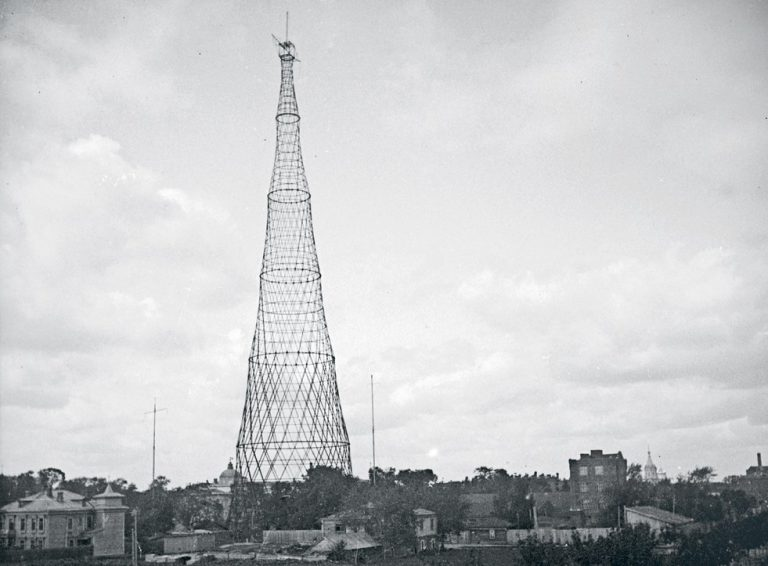
\includegraphics[width=1\textwidth]{images/tower-1}

		\end{column}
	\end{columns}
\end{frame}

%================================ 2
\begin{frame}{}

		Изначально задумывалась как телевизионная башня построена по проекту академика Владимира Григорьевича Шухова в период 1919-1922 годов. Проект телебашни на Шаболовке конструктор разработал в 1919 году.

\end{frame}


%================================ 3
\begin{frame}{}
		По первоначальному плану сооружение должно было быть 350-метровым и превзойти известную на весь мир Эйфелеву башню.
	\begin{columns}
		\begin{column}{0.3\textwidth}

			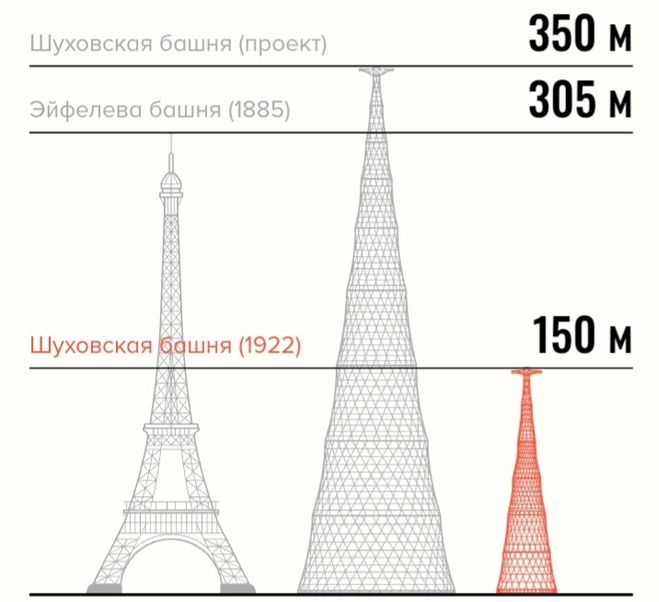
\includegraphics[width=1.3\textwidth]{images/tower-2}

		\end{column}


		\begin{column}{0.5\textwidth}

			%Но из-за разрухи, царившей после Октябрьской революции в Союзе, пришлось снизить завышенную планку. Катастрофически не хватало стали для сооружения объекта.
			В процессе строительства высоту телебашни уменьшили до 150 метров.

		\end{column}
	\end{columns}



\end{frame}


%================================ 4
\begin{frame}{Особенности конструкции}

	Архитектура строения - гиперболоидная конструкция в виде стальной сетчатой оболочки представленной в виде перекрещивающихся между собой прямых стальных профилей. Эти профили базируются на прочных основаниях – кольцах, создавая четкий геометрический рисунок – сетку.

\end{frame}


%================================ 5
\begin{frame}{}
	\begin{columns}
		\begin{column}{0.55\textwidth}
			Сетчатое сооружение обладает неоценимым достоинством – нагрузка ветра на нее сведена к минимуму.
\newline

			Простота и практичность чувствуется во всем, детали не требовали особой разработки и представляли собой заклепки и профили.
		\end{column}

		\begin{column}{0.45\textwidth}

			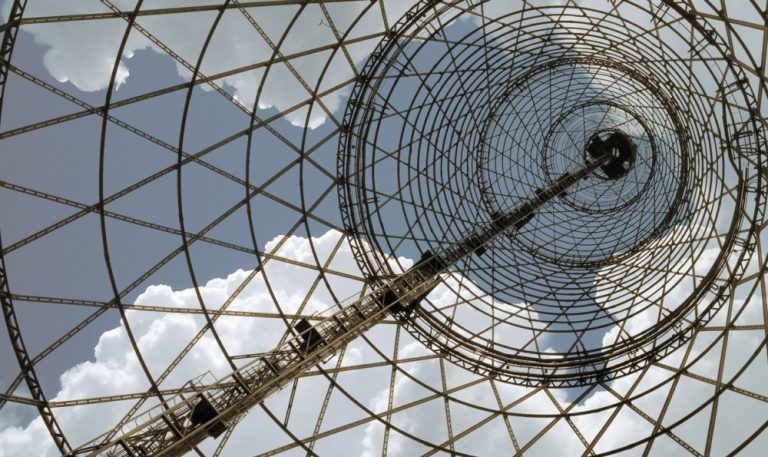
\includegraphics[width=0.9\textwidth]{images/tower-3}

		\end{column}
	\end{columns}
\end{frame}


%================================ 6
\begin{frame}{}
	Башня состояла из 6 секций по 25 метров в длину. Каждая секция была собрана внизу после чего с помощью специальных лебедок поднималась на свое место.
\end{frame}


%================================ 7
\begin{frame}{}
	Радиопередачи Шуховская башня начала сразу же после постройки. Первые же телепередачи жители Москвы увидели только в 1939 году.

	С началом Великой Отечественной войны трансляции прекратились. Башня вновь превратилась столичный радиопередатчик. В год победы телевидение вновь вернулось в Советский Союз.
\end{frame}


%================================ 8
\begin{frame}{}
	Трансляции с Шуховской башни были прекращены в 2002 году. Территория, на которой она находится, считается закрытой. Попасть на площадку можно только после специально выданного разрешения.
\end{frame}

%================================ 9
\begin{frame}{}
	За время своего существования Шуховская башня ни разу не подвергалась полноценной рестоврации. В 2003 году был утвержден фонд "Шуховская башня" который возглавил правнук инженера -- Владимир Шухов.
\end{frame}


%================================ 10
\begin{frame}{}
	На эти цели было выделено 135 млн. рублей. Этих средств оказалось не достаточно и работы отложили.

	Летом 2014 года москвичи путем референдума высказались за сохранение Шуховской башни. С целью безопасности была снята «антенная» секция.
\end{frame}


%================================ 11
\begin{frame}{}
	В январе 2017 года была заказана разработка проектной документации по реконструкции памятника. Цена контракта – более 32 миллионов рублей.
\end{frame}


\section{Благоданость}
\begin{frame}
	\centering
	\huge
	Спасибо за внимание!
\end{frame}


\end{document}
